\chapter{Implementation}
The chapter will explain how the different software are connected and what information is sent between them. All the configuration and start up commands can be found in the appendix.
\section{Software implementation}
The software implementation consist mainly of rtklib and dune. Piksi is also used in the experiment, however it's rtklib and the Dune task RTKGPS that will be discussed thoroughly.
\subsection{Rtkgps}
The \gls{rtk-gps} module in the navigation system consist of three parts. That is rtklib, and the two Dune tasks RTKGPS and Piksi. The RTKGPS task is connected to rtklib though a virtual connection, and the Piksi task has a physical connection to the Piksi receiver.


Rtklib is separated into the base station and the rover. The base station implementation runs the app str2str were it communicate with the ublox over a uart cable, and start up a tcp server.

The rover uses the rtkrcv app from rtklib to estimate the position of the rover. Rtkrcv connect itself as a tcp client to the tcp server that str2str create. Rtkrcv is configured in a moving baseline configuration to simulate the behavior that is expected during a landing on a ship. (Referer her til teori kap om rtklib)

The output from the Dune tasks is a \gls{imc} message called RtkFix, see table \ref{Tb:RtkFix}, which include the relative position of the \gls{uav} as well as the velocity, type of integer solution and the \gls{gps} \gls{tow}.
\begin{table}[!h]
\begin{center}
    \begin{tabular}{ | l | l |}
    \hline
    \textbf{Header} & \textbf{Content} \\ \hline
     tow & Gps time of Week  \\ \hline
     n & Baseline North coordinate \\ \hline
     e & Baseline East coordinate \\ \hline
     d & Baseline Down coordinate \\ \hline
     v\verb=_=n & Velocity North coordinate \\ \hline
     v\verb=_=e & Velocity East coordinate \\ \hline
     v\verb=_=d & Velocity Down coordinate \\ \hline
     iar\verb=_=hyp & Number of hypotheses in the Integer Ambiguity Resolution \\ \hline
     iar\verb=_=ratio & Quality ratio of Integer Ambiguity Resolution \\ \hline
     type & Type of fix: \\& None = No solution, but RTK task is running
     \\& Obs = No solution, but receiving observations
     \\& Float = Floating point solution of Integer Ambiguity Resolution
     \\& Fix = Fixed(single) solution of Integer Ambiguity Resolution \\ \hline
    \end{tabular}
\end{center}
\caption{The \gls{imc} message RtkFix }
\label{Tb:RtkFix}
\end{table}

\section{Hardware implementation}
The embedded computer uses GLUED as its operating system, and on it runs both Dune and rtklib. The Piksi and Ublox is connected to the BeagleBone over uart cables.

The primary data-link to the \gls{uav} is done with {shf} Ubiquiti AirMax radios, that is based on a Ubiquity Rocket M5
Has a WIFI connection to the base station.


The two \gls{rtk-gps} system is connected to a antenna splitter , figure \ref{figure:AntennaSplitter}, such that both system receive the same \gls{gnss} signals.

\begin{figure}[H]
	\centering
		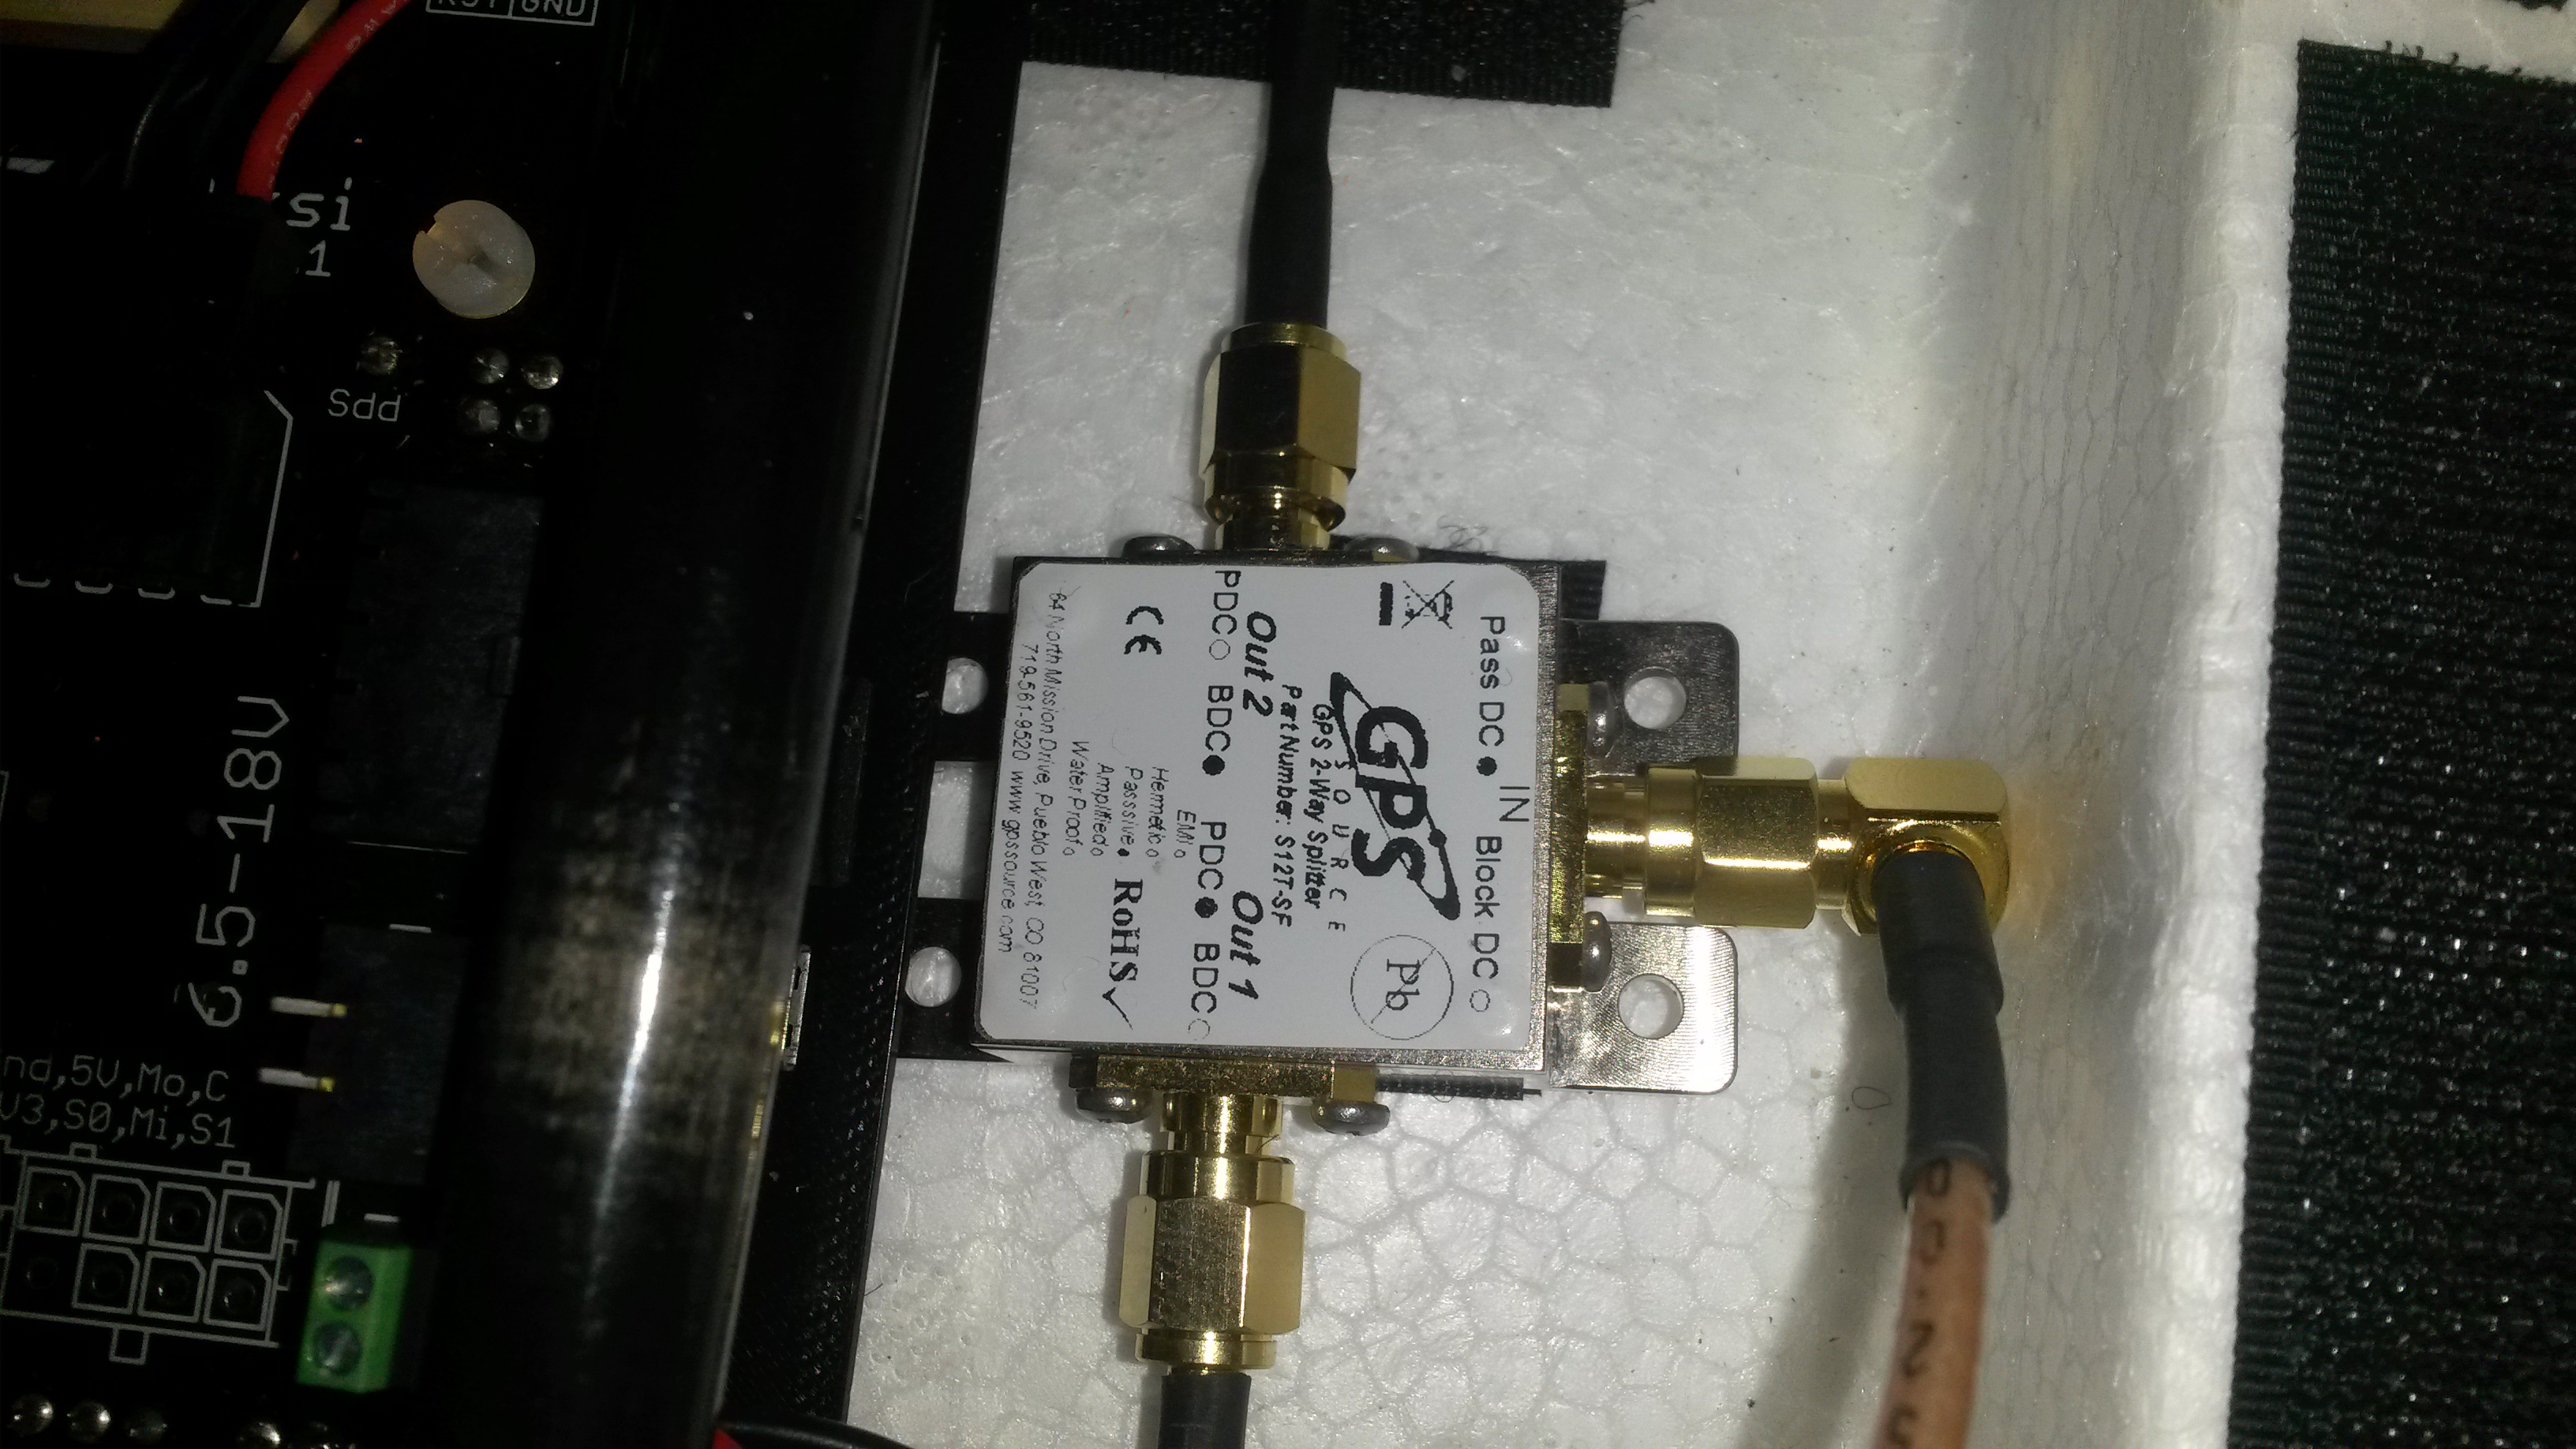
\includegraphics[width=0.7\textwidth]{figs/066.jpg}
		\caption{Antenna splitter}
		\label{figure:AntennaSplitter}
\end{figure}

This section contain how all the physical components are connected at both the rover and the base station. Include also how everything was prepared.

About Beaglebone: What runs on the beaglebone, connections, devices, what is it place in the system

About Ublox: Explain the ublox from a system perspective, how it's connected

Pixhawk: What do it do in the system:

Piksi: Same as ublox

The X8: How do it fit in the system

The base station: Same as x8

Antennas: 

Wifi router

